%!TEX root = ../main.tex
\chapter{Equazioni e sistemi non lineari}

La complessità di un problema, o il comportamento fisico di un sistema, può essere tale da non poter essere catturata da un modello lineare.
Si deve quindi ricorrere a modelli non lineari, che sono di più difficile trattazione.

\textit{Esempio.}
Supponiamo di avere un gas a una temperatura $T$ soggetto a una pressione $p$. Vogliamo calcolare il suo volume $V$. L'equazione dei gas è:
\begin{equation*}
\left[ p+a\left(\frac{N}{V}\right)^{2}\right]( V-Nb) =kNT
\end{equation*}
dove $a,b$ sono costanti che dipendono dal gas, $N$ è il numero di molecole, e $k$ è costante di Boltzmann. Per trovare $V$ dobbiamo dunque risolvere un'equazione non lineare.

È anche possibile che un'equazione non lineare emerga dall'applicazione di un metodo numerico implicito, come abbiamo visto nelle pagine precedenti.

\textit{Esempio.}
Consideriamo l'equazione differenziale
\begin{equation*}
\begin{cases}
y'(t) =\frac{y^{2}(t)}{t} ,\ t >1\\
y(1) =\dotsc
\end{cases}
\end{equation*}
Discretizzando questo problema con il metodo di \eqref{eq:eulero-indietro} otteniamo:
\begin{equation*}
u_{n+1} =u_{n} +h\left[\frac{( u_{n+1})^{2}}{t_{n+1}}\right] ,\quad n=0,1,2,\dotsc
\end{equation*}
Ad ogni passo temporale dobbiamo quindi risolvere un'equazione non lineare.

La risoluzione di equazioni non lineari avviene attraverso l'individuazione degli zeri di opportune funzioni.
Data una funzione $f$ reale di variabile reale, vogliamo trovare, \textit{se esistono}, i suoi zeri, ovvero cerchiamo $\alpha $ tale che $f( \alpha ) =0$.

\section{Metodo di bisezione}
\index{bisezione}
Per iniziare, ricordiamo un risultato di Analisi I.
\begin{theorem}
[di Bolzano]\index{teorema!di Bolzano}
Sia $f:[ a,b]\rightarrow \mathbb{R}$ continua e tale che $f(a) f(b) < 0$.
Allora esiste almeno un punto $\alpha \in ( a,b)$ tale che $f( \alpha ) =0$.
\end{theorem}

\textbf{NB.}
È importante che l'intervallo sia chiuso e limitato e ricordarsi che il teorema garantisce l'esistenza di \textit{almeno} uno zero, ma non ne fornisce il numero esatto.

Per applicare numericamente questo risultato, costruiamo dei metodi iterativi. Scegliamo $x^{(0)} \in [ a,b]$ e costruiamo una successione
$$ x^{(1)} ,x^{(2)} ,\dotsc ,x^{(k)} \quad \text{tale che} \quad \lim\limits _{k\rightarrow \infty } x^{(k)} =\alpha. $$

Operativamente, procediamo con gli stessi passi della dimostrazione del teorema di Bolzano, definiamo:
$$ a^{(0)} =a,b^{(0)} =b,I^{(0)} =\left[ a^{(0)} ,b^{(0)}\right] ,x^{(0)} =\frac{a^{(0)} +b^{(0)}}{2}.$$
Si presentano tre casi possibili:
\begin{itemize}
\item Se $f\left( x^{(0)}\right) =0$ abbiamo finito, $\alpha =x^{(0)}$.
\item Se $f\left( a^{(0)}\right) f\left( x^{(0)}\right) < 0$ allora $\alpha \in \left( a^{(0)} ,x^{(0)}\right)$ quindi ridefiniamo:
$$ a^{(1)} =a^{(0)} ,b^{(1)} =x^{(0)} ,I^{(1)} =\left( a^{(1)} ,b^{(1)}\right) ,x^{(1)} =\frac{a^{(1)} +b^{(1)}}{2}. $$
\item Se $f\left( x^{(0)}\right) f\left( b^{(0)}\right) < 0$ allora $\alpha \in \left( x^{(0)} ,b^{(0)}\right)$ quindi ridefiniamo:
$$ a^{(1)} =x^{(0)} ,b^{(1)} =b^{(0)} ,I^{(1)} =\left( a^{(1)} ,b^{(1)}\right) ,x^{(1)} =\frac{a^{(1)} +b^{(1)}}{2}. $$
\end{itemize}

Questo procedimento ricorsivo diventa l'\textbf{algoritmo di bisezione}.

\begin{algo}
	inizializza $a^{(0)} =a$\;
	inizializza $b^{(0)} =b$\;
	inizializza $x^{(0)} =\frac{a^{(0)} +b^{(0)}}{2}$\;
	\For{$k=0,1,2,\dotsc$}{
		\uIf{$f( x^{(k)}) =0$}{
			$\alpha =x^{(k)}$\;
			termina algoritmo\;
		}
		\uElseIf{$f( a^{(k)}) f( x^{(k)}) < 0$}{
			$a^{( k+1)} =a^{(k)}$\;
			$b^{( k+1)} =x^{(k)}$\;
			$x^{( k+1)} =\frac{a^{( k+1)} +b^{( k+1)}}{2}$\;
		}
		\ElseIf{$f( x^{(k)}) f( b^{(k)}) < 0$}{
			$a^{( k+1)} =x^{(k)}$\;
			$b^{( k+1)} =b^{(k)}$\;
			$x^{( k+1)} =\frac{a^{( k+1)} +b^{( k+1)}}{2}$\;
		}
		\If{criterio di arresto}{
			termina algoritmo\;
		}
	}
	\caption{Algoritmo di bisezione}
\end{algo}

\textit{Osservazioni.}
\begin{enumerate}
\item Ad ogni passo $k$, si ha che $\alpha \in I^{(k)} =\left[ a^{(k)} ,b^{(k)}\right]$. Inoltre:
\begin{equation*}
\left| I^{(k)}\right| =\left| b^{(k)} -a^{(k)}\right| =\frac{1}{2}\left| b^{( k-1)} -a^{( k-1)}\right| =\dotsc =\frac{1}{2^{k}}( b-a).
\end{equation*}
Quindi l'errore $e^{(k)} =x^{(k)} -\alpha $ può essere stimato come
\begin{equation*}
\left| e^{(k)}\right| =\left| x^{(k)} -\alpha \right| \leqslant \frac{1}{2}\left( b^{(k)} -a^{(k)}\right) =\frac{1}{2} I^{(k)} =\frac{1}{2^{k+1}}( b-a),
\end{equation*}
pertanto:
\begin{equation*}
0\leqslant \left| e^{(k)}\right| \leqslant \frac{1}{2^{k+1}}( b-a) \Rightarrow \lim _{k\rightarrow \infty }\left| e^{(k)}\right| =0.
\end{equation*}
\item Supponiamo di voler calcolare l'errore a meno di una precisione $\varepsilon$, cioè garantire che $\left| e^{(k)}\right| \leqslant \varepsilon$.
Calcoliamo l'iterazione $k_{\text{min}}$ prima della quale non possiamo interrompere il metodo:
\begin{align*}
\left| e^{(k)}\right| \leqslant \frac{1}{2^{k+1}}( b-a) & \leqslant \varepsilon \\
\frac{1}{2^{k+1}} & \leqslant \frac{\varepsilon }{b-a}\\
\log_{2}\frac{1}{2^{k+1}} & \leqslant \log_{2}\frac{\varepsilon }{b-a}\\
-( k+1) & \leqslant \log_{2}\frac{\varepsilon }{b-a}\\
k+1 & \geqslant -\log_{2}\frac{\varepsilon }{b-a}\\
k & \geqslant -\log_{2}\frac{\varepsilon }{b-a} -1\\
k & \geqslant \log_{2}\frac{b-a}{\varepsilon } -1,
\end{align*}
ovvero:
\begin{equation*}
k_{\text{min}} =\left\lceil \log_{2}\frac{b-a}{\varepsilon } -1\right\rceil
\end{equation*}
\end{enumerate}

% \textit{[Lezione 23 (19-05-2020)]}

Analizziamo la figura \ref{fig:osservazione-errore-non-monotono}: si può notare come al passo $0$ la soluzione sia molto vicina allo zero della funzione. Al passo $1$, in cui eliminiamo l'intervallo di sinistra, ci allontaniamo notevolmente rispetto all'iterazione precedente.

\begin{figure}[htpb]
	\centering
	\tikzset{every picture/.style={line width=0.75pt}} %set default line width to 0.75pt

	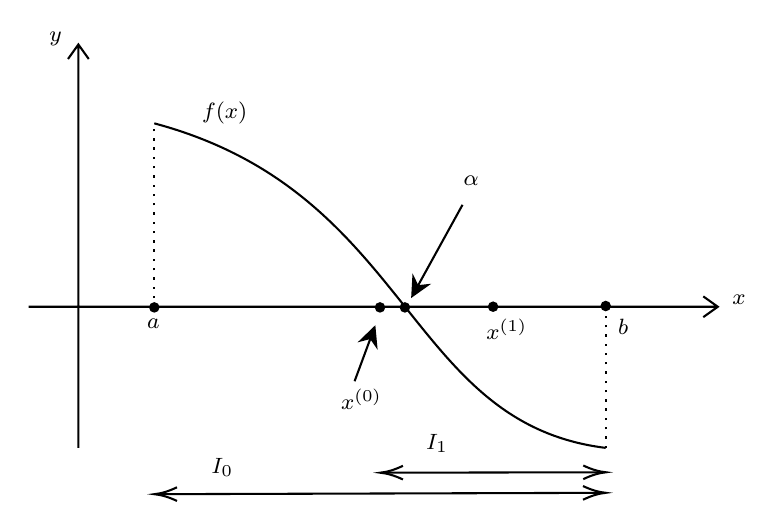
\begin{tikzpicture}[x=0.75pt,y=0.75pt,yscale=-1,xscale=1]
	%uncomment if require: \path (0,253); %set diagram left start at 0, and has height of 253

	%Shape: Axis 2D [id:dp33533961877243534]
	\draw  (133.5,142.36) -- (465.5,142.36)(157.43,16) -- (157.43,210.36) (458.5,137.36) -- (465.5,142.36) -- (458.5,147.36) (152.43,23) -- (157.43,16) -- (162.43,23)  ;
	%Curve Lines [id:da20121558433876752]
	\draw    (194,54) .. controls (318.5,87.34) and (314.5,198.34) .. (411.5,210.36) ;
	%Straight Lines [id:da9661795821517285]
	\draw  [dash pattern={on 0.84pt off 2.51pt}]  (194,142.67) -- (194,54) ;
	%Straight Lines [id:da4873438279286455]
	\draw  [dash pattern={on 0.84pt off 2.51pt}]  (411.5,210.36) -- (411.5,142) ;
	%Straight Lines [id:da9946674756730165]
	\draw    (304.86,222.31) -- (409.61,222.11) ;
	\draw [shift={(411.61,222.11)}, rotate = 539.9] [color={rgb, 255:red, 0; green, 0; blue, 0 }  ][line width=0.75]    (10.93,-3.29) .. controls (6.95,-1.4) and (3.31,-0.3) .. (0,0) .. controls (3.31,0.3) and (6.95,1.4) .. (10.93,3.29)   ;
	\draw [shift={(302.86,222.31)}, rotate = 359.9] [color={rgb, 255:red, 0; green, 0; blue, 0 }  ][line width=0.75]    (10.93,-3.29) .. controls (6.95,-1.4) and (3.31,-0.3) .. (0,0) .. controls (3.31,0.3) and (6.95,1.4) .. (10.93,3.29)   ;
	%Shape: Circle [id:dp8374417825384726]
	\draw  [fill={rgb, 255:red, 0; green, 0; blue, 0 }  ,fill opacity=1 ] (192,142.67) .. controls (192,141.56) and (192.9,140.67) .. (194,140.67) .. controls (195.1,140.67) and (196,141.56) .. (196,142.67) .. controls (196,143.77) and (195.1,144.67) .. (194,144.67) .. controls (192.9,144.67) and (192,143.77) .. (192,142.67) -- cycle ;
	%Shape: Circle [id:dp032665240645063376]
	\draw  [fill={rgb, 255:red, 0; green, 0; blue, 0 }  ,fill opacity=1 ] (300.75,142.67) .. controls (300.75,141.56) and (301.65,140.67) .. (302.75,140.67) .. controls (303.85,140.67) and (304.75,141.56) .. (304.75,142.67) .. controls (304.75,143.77) and (303.85,144.67) .. (302.75,144.67) .. controls (301.65,144.67) and (300.75,143.77) .. (300.75,142.67) -- cycle ;
	%Shape: Circle [id:dp9304288736660509]
	\draw  [fill={rgb, 255:red, 0; green, 0; blue, 0 }  ,fill opacity=1 ] (312.75,142.67) .. controls (312.75,141.56) and (313.65,140.67) .. (314.75,140.67) .. controls (315.85,140.67) and (316.75,141.56) .. (316.75,142.67) .. controls (316.75,143.77) and (315.85,144.67) .. (314.75,144.67) .. controls (313.65,144.67) and (312.75,143.77) .. (312.75,142.67) -- cycle ;
	%Shape: Circle [id:dp9634240894311528]
	\draw  [fill={rgb, 255:red, 0; green, 0; blue, 0 }  ,fill opacity=1 ] (409.5,142) .. controls (409.5,140.9) and (410.4,140) .. (411.5,140) .. controls (412.6,140) and (413.5,140.9) .. (413.5,142) .. controls (413.5,143.1) and (412.6,144) .. (411.5,144) .. controls (410.4,144) and (409.5,143.1) .. (409.5,142) -- cycle ;
	%Shape: Circle [id:dp1350212381008955]
	\draw  [fill={rgb, 255:red, 0; green, 0; blue, 0 }  ,fill opacity=1 ] (355.24,142.33) .. controls (355.24,141.23) and (356.13,140.33) .. (357.24,140.33) .. controls (358.34,140.33) and (359.24,141.23) .. (359.24,142.33) .. controls (359.24,143.44) and (358.34,144.33) .. (357.24,144.33) .. controls (356.13,144.33) and (355.24,143.44) .. (355.24,142.33) -- cycle ;
	%Straight Lines [id:da07104153441328442]
	\draw    (196,232.66) -- (409.5,232.01) ;
	\draw [shift={(411.5,232)}, rotate = 539.8199999999999] [color={rgb, 255:red, 0; green, 0; blue, 0 }  ][line width=0.75]    (10.93,-3.29) .. controls (6.95,-1.4) and (3.31,-0.3) .. (0,0) .. controls (3.31,0.3) and (6.95,1.4) .. (10.93,3.29)   ;
	\draw [shift={(194,232.67)}, rotate = 359.82] [color={rgb, 255:red, 0; green, 0; blue, 0 }  ][line width=0.75]    (10.93,-3.29) .. controls (6.95,-1.4) and (3.31,-0.3) .. (0,0) .. controls (3.31,0.3) and (6.95,1.4) .. (10.93,3.29)   ;
	%Straight Lines [id:da08740253227174466]
	\draw    (342.5,93.25) -- (319.2,135.54) ;
	\draw [shift={(317.75,138.17)}, rotate = 298.86] [fill={rgb, 255:red, 0; green, 0; blue, 0 }  ][line width=0.08]  [draw opacity=0] (10.72,-5.15) -- (0,0) -- (10.72,5.15) -- (7.12,0) -- cycle    ;
	%Straight Lines [id:da9937908466011312]
	\draw    (290.5,178.25) -- (299.46,154.06) ;
	\draw [shift={(300.5,151.25)}, rotate = 470.32] [fill={rgb, 255:red, 0; green, 0; blue, 0 }  ][line width=0.08]  [draw opacity=0] (10.72,-5.15) -- (0,0) -- (10.72,5.15) -- (7.12,0) -- cycle    ;

	% Text Node
	\draw (215.5,42.4) node [anchor=north west][inner sep=0.75pt]  [font=\footnotesize]  {$f(x)$};
	% Text Node
	\draw (471,135.4) node [anchor=north west][inner sep=0.75pt]  [font=\footnotesize]  {$x$};
	% Text Node
	\draw (142,8.4) node [anchor=north west][inner sep=0.75pt]  [font=\footnotesize]  {$y$};
	% Text Node
	\draw (341.5,77.9) node [anchor=north west][inner sep=0.75pt]  [font=\footnotesize]  {$\alpha $};
	% Text Node
	\draw (220,213.9) node [anchor=north west][inner sep=0.75pt]  [font=\footnotesize]  {$I_{0}$};
	% Text Node
	\draw (323.5,202.4) node [anchor=north west][inner sep=0.75pt]  [font=\footnotesize]  {$I_{1}$};
	% Text Node
	\draw (189,146.9) node [anchor=north west][inner sep=0.75pt]  [font=\footnotesize]  {$a$};
	% Text Node
	\draw (416,146.9) node [anchor=north west][inner sep=0.75pt]  [font=\footnotesize]  {$b$};
	% Text Node
	\draw (282.5,180.4) node [anchor=north west][inner sep=0.75pt]  [font=\footnotesize]  {$x^{(0)}$};
	% Text Node
	\draw (352.5,146.9) node [anchor=north west][inner sep=0.75pt]  [font=\footnotesize]  {$x^{(1)}$};
	\end{tikzpicture}
	\caption{L'errore col metodo di bisezione non tende a zero in modo monotono.}
	\label{fig:osservazione-errore-non-monotono}
\end{figure}
\FloatBarrier

In generale, la successione degli errori $e^{(k)}$ generata dal metodo di bisezione non converge a zero \textit{monotonicamente}.
\begin{definition}
[Ordine di convergenza]
\index{ordine!di convergenza}
Sia $\left\{x^{(k)}\right\}_{k\geqslant 0}$ la successione di approssimazioni di $\alpha $ generata da un metodo numerico. Diciamo che la successione converge ad $\alpha $ con ordine $p$, con $\geqslant 1$, se esiste $C >0$ tale che
\begin{equation*}
\frac{\left| x^{( k+1)} -\alpha \right| }{\left| x^{(k)} -\alpha \right| ^{p}} \leqslant C,\quad \forall k\geqslant k_{0} ,\quad k_{0} \in \mathbb{Z}_{+} \cup \{0\} .
\end{equation*}
Se $p=1$, per avere convergenza deve essere $C< 1$, e in questo caso $C$ è detto \textbf{fattore di convergenza}\index{fattore di convergenza}.
\end{definition}
Vogliamo costruire dei metodi numerici che garantiscano convergenza secondo questa definizione.
\section{Approccio geometrico per l'approssimazione di radici}

L'idea è di fare uno sviluppo di Taylor nell'intorno del punto $x$:
\begin{equation*}
0 =f( \alpha ) =f( x+( \alpha -x)) = f(x) +( \alpha -x) f'( \xi ).
\end{equation*}
Se pensiamo la soluzione $\alpha$ come l'iterata successiva $x^{( k+1)}$ e $x$ come il punto nel quale il metodo si trova attualmente, otteniamo la struttura del metodo iterativo:
\begin{equation*}
f\left( x^{(k)}\right) +\left( x^{( k+1)} -x^{(k)}\right) f'( \xi ) =0.
\end{equation*}
Si noti che il punto $\xi $ non è noto, altrimenti basterebbe un solo passo, calcolando la derivata della funzione in $\xi$ e arrivando direttamente ad $\alpha $.
Per questa ragione, sostituiamo il termine $f'( \xi )$ con $q^{(k)}$, la cui scelta caratterizzerà il metodo numerico e determinerà la velocità con cui esso arriverà ad $\alpha $:
\begin{equation*}
\begin{aligned}
f\left( x^{(k)}\right) +\left( x^{( k+1)} -x^{(k)}\right) q^{(k)} & =0\\
\left( x^{( k+1)} -x^{(k)}\right) q^{(k)} & =-f\left( x^{(k)}\right)\\
x^{( k+1)} -x^{(k)} & =-\frac{f\left( x^{(k)}\right)}{q^{(k)}}\\
x^{( k+1)} & =x^{(k)} -\frac{f\left( x^{(k)}\right)}{q^{(k)}}.
\end{aligned}
\end{equation*}
La forma generale è quindi:
\begin{equation}
x^{( k+1)} =x^{(k)} -\frac{1}{q^{(k)}} f\left( x^{(k)}\right) ,\ \ \forall k\geqslant 0.
\label{eq:forma-generale-non-lineari}
\end{equation}

Vediamo ora tre metodi per approssimare le radici:
\begin{itemize}
	\item \textbf{Metodo di Newton}\index{metodo!di Newton}:
		Supponiamo $f\in C^{1}( a,b)$ e $f'(x)\neq 0, \forall x \in (a,b)$, scegliamo
		\begin{equation*}
		q^{(k)} =f'\left( x^{(k)}\right) ,\ \ \forall k\geqslant 0,
		\end{equation*}
		allora \eqref{eq:forma-generale-non-lineari} diventa:
		\begin{equation*}
		x^{( k+1)} =x^{(k)} -\frac{f\left( x^{(k)}\right)}{f'\left( x^{(k)}\right)} ,\ \ \forall k\geqslant 0.
		\end{equation*}
	\item \textbf{Metodo delle secanti}\index{metodo!delle secanti}:
		Per il metodo delle secanti, scegliamo invece
		\begin{equation*}
		q^{(k)} =\frac{f\left( x^{(k)}\right) -f\left( x^{(k-1)}\right)}{x^{(k)} -x^{(k-1)}} ,\ \ \forall k\geqslant 1,
		\end{equation*}
		allora \eqref{eq:forma-generale-non-lineari} diventa:
		\begin{equation*}
		x^{(k+1)} =x^{(k)} -\frac{x^{(k)} -x^{(k-1)}}{f\left( x^{(k)}\right) -f\left( x^{(k-1)}\right)} f\left( x^{(k)}\right) ,\ \ \forall k\geqslant 1.
		\end{equation*}
	\item \textbf{Metodo delle corde}\index{metodo!delle corde}:
		Il metodo delle corde usa:
		\begin{equation*}
		q^{(k)} =q=\frac{f(b)-f(a)}{b-a} ,\ \ \forall k\geqslant 0,
		\end{equation*}
		quindi \eqref{eq:forma-generale-non-lineari} diventa:
		\begin{equation*}
		x^{(k+1)} =x^{(k)} -\frac{b-a}{f(b)-f(a)} f\left( x^{(k)}\right) ,\ \ \forall k\geqslant 0.
		\end{equation*}
\end{itemize}

\textbf{NB.}
I metodi descritti convergono \textit{localmente} rispetto alla definizione che ci siamo dati, ovvero è importante che il dato iniziale $x^{(0)}$ sia scelto ragionevolmente vicino allo zero esatto della funzione. Diversamente dai metodi iterativi per sistemi lineari, qui la scelta del dato iniziale è importante.

\section{Metodo delle iterazioni di punto fisso}
Vediamo un modo più generale di vedere gli algoritmi per equazioni non lineari.
A questo scopo, sia $\alpha $ tale che $f( \alpha ) =0$. Se definiamo:
\begin{equation}
	\Phi ( x) \coloneqq x-f( x) ,
\end{equation}
allora risulta che $\alpha $ è un \textbf{punto fisso}\index{punto fisso} di $\Phi ( x)$, infatti:
\begin{equation*}
	\Phi ( \alpha ) =\alpha -\underbrace{f( \alpha )}_{=0} =\alpha,
\end{equation*}
quindi cercare gli zeri di $f$ è equivalente a cercare i punti fissi della cosiddetta \textbf{funzione di iterazione}\index{funzione!di iterazione} $\Phi ( x)$.

L'idea è di calcolare ogni iterata come la funzione di iterazione valutata all'iterata precedente:
\begin{equation}
	x^{( k+1)} =\Phi \big( x^{(k)}\big) ,\ \ k\geqslant 0,
	\label{eq:iterazioni-punto-fisso}
\end{equation}
e si prosegue fino a convergenza.

L'algoritmo è pertanto il seguente.

\begin{algo}
	inizializza $\x^{(0)}$\;
	\For{$k=0,1,\dotsc$}{
		$x^{(k+1)} = \Phi\left( x^{(k)} \right)$\;
		\If{criterio di arresto}{
			termina algoritmo\;
		}
	}
	\caption{Algoritmo delle iterazioni di punto fisso.}
\end{algo}

L'approccio visivo si può osservare in figura \ref{fig:intuizione-punto-fisso}.

\begin{figure}[htpb]
	\centering
	\tikzset{every picture/.style={line width=0.75pt}} %set default line width to 0.75pt        

	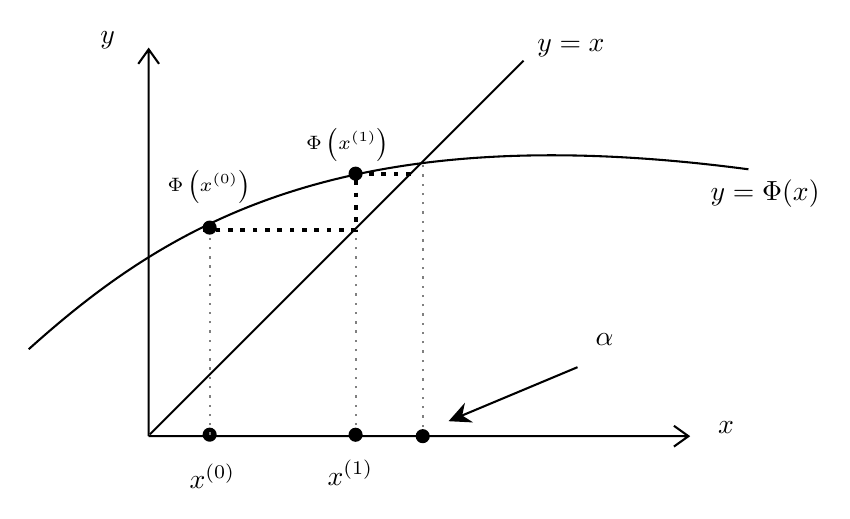
\begin{tikzpicture}[x=0.75pt,y=0.75pt,yscale=-1,xscale=1]
	%uncomment if require: \path (0,300); %set diagram left start at 0, and has height of 300

	%Shape: Axis 2D [id:dp3566775992086928] 
	\draw  (157.79,212.28) -- (417.86,212.28)(157.79,25.89) -- (157.79,212.28) -- cycle (410.86,207.28) -- (417.86,212.28) -- (410.86,217.28) (152.79,32.89) -- (157.79,25.89) -- (162.79,32.89)  ;
	%Curve Lines [id:da6752669888557952] 
	\draw    (100,170.38) .. controls (165.98,111.14) and (250.55,57.68) .. (446.76,83.69) ;
	%Straight Lines [id:da8869587279017774] 
	\draw [color={rgb, 255:red, 128; green, 128; blue, 128 }  ,draw opacity=1 ] [dash pattern={on 0.84pt off 2.51pt}]  (289.83,212.28) -- (289.83,81.24) ;
	%Straight Lines [id:da5511356307086455] 
	\draw [color={rgb, 255:red, 128; green, 128; blue, 128 }  ,draw opacity=1 ] [dash pattern={on 0.84pt off 2.51pt}]  (257.49,211.59) -- (257.49,112.82) ;
	%Shape: Circle [id:dp7693840113711456] 
	\draw  [fill={rgb, 255:red, 0; green, 0; blue, 0 }  ,fill opacity=1 ] (184.28,211.55) .. controls (184.28,209.96) and (185.58,208.66) .. (187.17,208.66) .. controls (188.77,208.66) and (190.06,209.96) .. (190.06,211.55) .. controls (190.06,213.15) and (188.77,214.44) .. (187.17,214.44) .. controls (185.58,214.44) and (184.28,213.15) .. (184.28,211.55) -- cycle ;
	%Shape: Ellipse [id:dp4236145004323377] 
	\draw  [fill={rgb, 255:red, 0; green, 0; blue, 0 }  ,fill opacity=1 ] (286.94,212.28) .. controls (286.94,210.68) and (288.23,209.39) .. (289.83,209.39) .. controls (291.42,209.39) and (292.72,210.68) .. (292.72,212.28) .. controls (292.72,213.87) and (291.42,215.17) .. (289.83,215.17) .. controls (288.23,215.17) and (286.94,213.87) .. (286.94,212.28) -- cycle ;
	%Shape: Ellipse [id:dp6046639245591658] 
	\draw  [fill={rgb, 255:red, 0; green, 0; blue, 0 }  ,fill opacity=1 ] (254.6,211.59) .. controls (254.6,210) and (255.89,208.7) .. (257.49,208.7) .. controls (259.08,208.7) and (260.38,210) .. (260.38,211.59) .. controls (260.38,213.19) and (259.08,214.48) .. (257.49,214.48) .. controls (255.89,214.48) and (254.6,213.19) .. (254.6,211.59) -- cycle ;
	%Straight Lines [id:da5989367722690591] 
	\draw    (364.4,179.04) -- (305.04,203.89) ;
	\draw [shift={(302.28,205.05)}, rotate = 337.28999999999996] [fill={rgb, 255:red, 0; green, 0; blue, 0 }  ][line width=0.08]  [draw opacity=0] (10.72,-5.15) -- (0,0) -- (10.72,5.15) -- (7.12,0) -- cycle    ;
	%Straight Lines [id:da8569096885462997] 
	\draw    (338.4,31.37) -- (158.42,211.35) ;
	%Straight Lines [id:da14498326366026926] 
	\draw [line width=1.5]  [dash pattern={on 1.69pt off 2.76pt}]  (283.97,85.79) -- (257.49,85.79) -- (257.49,112.82) -- (182.36,112.82) ;
	%Straight Lines [id:da6377659143246175] 
	\draw [color={rgb, 255:red, 128; green, 128; blue, 128 }  ,draw opacity=1 ] [dash pattern={on 0.84pt off 2.51pt}]  (187.17,211.55) -- (187.17,111.79) ;
	%Shape: Ellipse [id:dp979569157625213] 
	\draw  [fill={rgb, 255:red, 0; green, 0; blue, 0 }  ,fill opacity=1 ] (184.28,111.79) .. controls (184.28,110.2) and (185.58,108.9) .. (187.17,108.9) .. controls (188.77,108.9) and (190.06,110.2) .. (190.06,111.79) .. controls (190.06,113.39) and (188.77,114.68) .. (187.17,114.68) .. controls (185.58,114.68) and (184.28,113.39) .. (184.28,111.79) -- cycle ;
	%Shape: Ellipse [id:dp09526697663217876] 
	\draw  [fill={rgb, 255:red, 0; green, 0; blue, 0 }  ,fill opacity=1 ] (254.6,85.79) .. controls (254.6,84.19) and (255.89,82.9) .. (257.49,82.9) .. controls (259.08,82.9) and (260.38,84.19) .. (260.38,85.79) .. controls (260.38,87.38) and (259.08,88.68) .. (257.49,88.68) .. controls (255.89,88.68) and (254.6,87.38) .. (254.6,85.79) -- cycle ;

	% Text Node
	\draw (427.1,87.42) node [anchor=north west][inner sep=0.75pt]  [font=\normalsize]  {$y=\Phi ( x)$};
	% Text Node
	\draw (430.64,203.79) node [anchor=north west][inner sep=0.75pt]  [font=\normalsize]  {$x$};
	% Text Node
	\draw (133.01,15.96) node [anchor=north west][inner sep=0.75pt]  [font=\normalsize]  {$y$};
	% Text Node
	\draw (371.63,161.33) node [anchor=north west][inner sep=0.75pt]  [font=\normalsize]  {$\alpha $};
	% Text Node
	\draw (176.04,224.16) node [anchor=north west][inner sep=0.75pt]  [font=\normalsize]  {$x^{( 0)}$};
	% Text Node
	\draw (242.5,222.48) node [anchor=north west][inner sep=0.75pt]  [font=\normalsize]  {$x^{( 1)}$};
	% Text Node
	\draw (343.52,19.51) node [anchor=north west][inner sep=0.75pt]  [font=\normalsize]  {$y=x$};
	% Text Node
	\draw (165.47,82.64) node [anchor=north west][inner sep=0.75pt]  [font=\scriptsize]  {$\Phi \left( x^{( 0)}\right)$};
	% Text Node
	\draw (232.21,62.45) node [anchor=north west][inner sep=0.75pt]  [font=\scriptsize]  {$\Phi \left( x^{( 1)}\right)$};


	\end{tikzpicture}
	\caption{Intuizione geometrica del metodo delle iterazioni di punto fisso.}
	\label{fig:intuizione-punto-fisso}
\end{figure}

È tuttavia facile pensare a dei controesempi in cui la funzione $\Phi $ non porta a convergenza, come in figura \ref{fig:punto-fisso-no-convergenza}. Tale problema sarà risolto nel teorema \ref{thm:ostrowski}.

\begin{figure}[htpb]
	\centering
	

	\tikzset{every picture/.style={line width=0.75pt}} %set default line width to 0.75pt        

	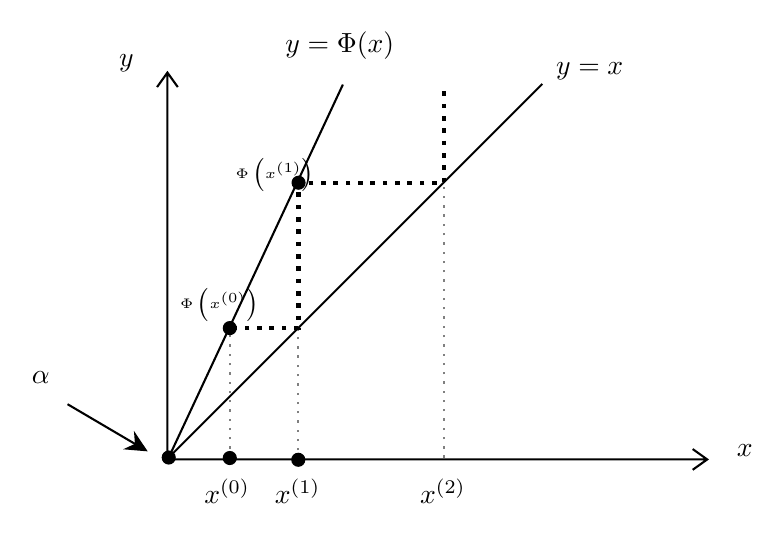
\begin{tikzpicture}[x=0.75pt,y=0.75pt,yscale=-1,xscale=1]
	%uncomment if require: \path (0,300); %set diagram left start at 0, and has height of 300

	%Shape: Axis 2D [id:dp1346140806136602] 
	\draw  (157.79,232.28) -- (417.86,232.28)(157.79,45.89) -- (157.79,232.28) -- cycle (410.86,227.28) -- (417.86,232.28) -- (410.86,237.28) (152.79,52.89) -- (157.79,45.89) -- (162.79,52.89)  ;
	%Straight Lines [id:da5286058801327398] 
	\draw [color={rgb, 255:red, 128; green, 128; blue, 128 }  ,draw opacity=1 ] [dash pattern={on 0.84pt off 2.51pt}]  (290.97,231.5) -- (290.97,98.96) ;
	%Straight Lines [id:da563386105754107] 
	\draw [color={rgb, 255:red, 128; green, 128; blue, 128 }  ,draw opacity=1 ] [dash pattern={on 0.84pt off 2.51pt}]  (187.84,231.59) -- (187.84,169) ;
	%Shape: Ellipse [id:dp6287751568639635] 
	\draw  [fill={rgb, 255:red, 0; green, 0; blue, 0 }  ,fill opacity=1 ] (155.53,231.35) .. controls (155.53,229.75) and (156.82,228.46) .. (158.42,228.46) .. controls (160.01,228.46) and (161.31,229.75) .. (161.31,231.35) .. controls (161.31,232.95) and (160.01,234.24) .. (158.42,234.24) .. controls (156.82,234.24) and (155.53,232.95) .. (155.53,231.35) -- cycle ;
	%Shape: Ellipse [id:dp21716140586002886] 
	\draw  [fill={rgb, 255:red, 0; green, 0; blue, 0 }  ,fill opacity=1 ] (184.95,231.59) .. controls (184.95,230) and (186.24,228.7) .. (187.84,228.7) .. controls (189.43,228.7) and (190.73,230) .. (190.73,231.59) .. controls (190.73,233.19) and (189.43,234.48) .. (187.84,234.48) .. controls (186.24,234.48) and (184.95,233.19) .. (184.95,231.59) -- cycle ;
	%Straight Lines [id:da4765382924209203] 
	\draw    (109.67,205.67) -- (145.69,226.86) ;
	\draw [shift={(148.28,228.39)}, rotate = 210.47] [fill={rgb, 255:red, 0; green, 0; blue, 0 }  ][line width=0.08]  [draw opacity=0] (10.72,-5.15) -- (0,0) -- (10.72,5.15) -- (7.12,0) -- cycle    ;
	%Straight Lines [id:da10658482700916871] 
	\draw    (338.4,51.37) -- (158.42,231.35) ;
	%Straight Lines [id:da1798774361287676] 
	\draw [line width=1.5]  [dash pattern={on 1.69pt off 2.76pt}]  (290.97,55) -- (290.97,98.96) -- (220.97,98.96) -- (220.97,169) -- (187.84,169) ;
	%Straight Lines [id:da4108558993374163] 
	\draw    (242.33,51.67) -- (158.42,231.35) ;
	%Shape: Ellipse [id:dp960624181595366] 
	\draw  [fill={rgb, 255:red, 0; green, 0; blue, 0 }  ,fill opacity=1 ] (184.95,169) .. controls (184.95,167.4) and (186.24,166.11) .. (187.84,166.11) .. controls (189.43,166.11) and (190.73,167.4) .. (190.73,169) .. controls (190.73,170.6) and (189.43,171.89) .. (187.84,171.89) .. controls (186.24,171.89) and (184.95,170.6) .. (184.95,169) -- cycle ;
	%Straight Lines [id:da06469788534794985] 
	\draw [color={rgb, 255:red, 128; green, 128; blue, 128 }  ,draw opacity=1 ] [dash pattern={on 0.84pt off 2.51pt}]  (220.84,232.44) -- (220.84,169.85) ;
	%Shape: Ellipse [id:dp29351931672149534] 
	\draw  [fill={rgb, 255:red, 0; green, 0; blue, 0 }  ,fill opacity=1 ] (217.95,232.44) .. controls (217.95,230.85) and (219.24,229.55) .. (220.84,229.55) .. controls (222.43,229.55) and (223.73,230.85) .. (223.73,232.44) .. controls (223.73,234.04) and (222.43,235.33) .. (220.84,235.33) .. controls (219.24,235.33) and (217.95,234.04) .. (217.95,232.44) -- cycle ;
	%Shape: Ellipse [id:dp30400825590060854] 
	\draw  [fill={rgb, 255:red, 0; green, 0; blue, 0 }  ,fill opacity=1 ] (218.08,98.96) .. controls (218.08,97.37) and (219.37,96.07) .. (220.97,96.07) .. controls (222.56,96.07) and (223.86,97.37) .. (223.86,98.96) .. controls (223.86,100.56) and (222.56,101.85) .. (220.97,101.85) .. controls (219.37,101.85) and (218.08,100.56) .. (218.08,98.96) -- cycle ;

	% Text Node
	\draw (213.1,24.76) node [anchor=north west][inner sep=0.75pt]  [font=\normalsize]  {$y=\Phi ( x)$};
	% Text Node
	\draw (430.64,223.79) node [anchor=north west][inner sep=0.75pt]  [font=\normalsize]  {$x$};
	% Text Node
	\draw (133.01,35.96) node [anchor=north west][inner sep=0.75pt]  [font=\normalsize]  {$y$};
	% Text Node
	\draw (90.96,188.66) node [anchor=north west][inner sep=0.75pt]  [font=\normalsize]  {$\alpha $};
	% Text Node
	\draw (174.04,240.16) node [anchor=north west][inner sep=0.75pt]  [font=\normalsize]  {$x^{( 0)}$};
	% Text Node
	\draw (343.52,39.51) node [anchor=north west][inner sep=0.75pt]  [font=\normalsize]  {$y=x$};
	% Text Node
	\draw (162.47,148.31) node [anchor=north west][inner sep=0.75pt]  [font=\tiny]  {$\Phi \left( x^{( 0)}\right)$};
	% Text Node
	\draw (189.21,85.79) node [anchor=north west][inner sep=0.75pt]  [font=\tiny]  {$\Phi \left( x^{( 1)}\right)$};
	% Text Node
	\draw (208.04,240.16) node [anchor=north west][inner sep=0.75pt]  [font=\normalsize]  {$x^{( 1)}$};
	% Text Node
	\draw (278.04,240.16) node [anchor=north west][inner sep=0.75pt]  [font=\normalsize]  {$x^{( 2)}$};


	\end{tikzpicture}
	\caption{Esempio in cui il metodo di punto fisso non porta a convergenza.}
	\label{fig:punto-fisso-no-convergenza}
\end{figure}

\textit{Osservazione.}
Il metodo delle corde e il metodo di Newton possono essere scritti come metodi di iterazione di punto fisso:
\begin{itemize}
\item Metodo delle corde:
\begin{equation*}
x^{(0)} ,\ \ x^{(k+1)} =\Phi _{\text{corde}}\left( x^{(k)}\right) \quad \text{con } \ \Phi _{\text{corde}}(x) =x-\frac{b-a}{f(b)-f(a)} f(x).
\end{equation*}
\item Metodo di Newton:
\begin{equation*}
x^{(k+1)} =\Phi _{\text{Newton}}\left( x^{(k)}\right) \quad \text{con  } \ \Phi _{\text{Newton}}(x) =x-\frac{f(x)}{f'(x)}.
\end{equation*}
\end{itemize}
\begin{theorem}
[Convergenza delle iterazioni di punto fisso]
\index{teorema!della convergenza delle iterazioni di punto fisso}
Consideriamo la successione delle iterazioni di punto fisso \eqref{eq:iterazioni-punto-fisso}.

Supponiamo che $\Phi $ sia continua in $[ a,b]$ e sia tale che $\Phi (x) \in [ a,b]$ per ogni $x\in [ a,b]$; allora esiste almeno un punto fisso $\alpha \in [ a,b]$.

Se supponiamo inoltre che $\Phi $ sia una contrazione, cioè che:
\begin{equation*}
\exists L< 1\ \text{t.c.} \ | \Phi ( x_{1}) -\Phi ( x_{2})| \leq L| x_{1} -x_{2}| \quad \forall x_{1} ,x_{2} \in [a,b].
\end{equation*}
Allora il punto fisso $\alpha$ è unico e la successione \eqref{eq:iterazioni-punto-fisso} converge ad $\alpha $, per qualunque scelta del dato iniziale $x^{(0)} \in [ a,b]$.
\end{theorem}

\begin{theorem}
[di Ostrowski]
\label{thm:ostrowski}
\index{teorema!di Ostrowski}
Sia $\alpha $ un punto fisso di una funzione $\Phi $ continua e derivabile con continuità in un opportuno intorno $I$ di $\alpha $. Se risulta $| \Phi '(\alpha )| < 1$, allora esiste $\delta  >0$ in tale che la successione $\left\{x^{(k)}\right\}$ converge ad $\alpha $, per ogni $x^{(0)}$ per cui si abbia $\left| x^{(0)} -\alpha \right| < \delta $. Inoltre:
\begin{equation*}
\lim _{k\rightarrow \infty }\frac{x^{(k+1)} -\alpha }{x^{(k)} -\alpha } =\Phi '(\alpha ).
\end{equation*}
\end{theorem}
La quantità $| \Phi '(\alpha )| $ è detta \textbf{fattore asintotico di convergenza}\index{fattore!asintotico di convergenza} e, in analogia con il caso dei metodi iterativi per la risoluzione di sistemi lineari, si definisce la \textbf{velocità asintotica di convergenza}\index{velocità!asintotica di convergenza} come segue:
\begin{equation*}
R=-\log(| \Phi '(\alpha )| ).
\end{equation*}
Ricapitolando:
\begin{itemize}
\item se $| \Phi '(\alpha )| < 1$ il metodo è localmente convergente. In particolare:
\begin{itemize}
\item se $\Phi '(\alpha ) >0$ le iterate si avvicinano ad $\alpha $ in maniera monotona;
\item se $\Phi '(\alpha )< 0$ le iterate si avvicinano ad $\alpha $ oscillando intorno ad $\alpha $;
\end{itemize}
\item se $| \Phi '(\alpha )|  >1$ il metodo è divergente;
\item se $| \Phi '(\alpha )| =1$ non è possibile trarre conclusioni dal teorema.
\end{itemize}
Vediamo ora un altro risultato notevole sui metodi di punto fisso.
\begin{theorem}
Se $\Phi \in C^{p+1} (I)$ per un opportuno intorno $I$ di $\alpha $ e per un intero $p\geqslant 1,$ e se $\Phi ^{(i)} (\alpha )=0$ per $i=1,\dotsc ,p$ mentre $\Phi ^{(p+1)} (\alpha )\neq 0,$ allora il metodo di punto fisso con funzione di iterazione $\Phi $ ha ordine $p+1$ e risulta inoltre che
\begin{equation*}
\lim _{k\rightarrow \infty }\frac{x^{(k+1)} -\alpha }{\left( x^{(k)} -\alpha \right)^{p+1}} =\frac{\Phi ^{(p+1)} (\alpha )}{(p+1)!}.
\end{equation*}
\end{theorem}

\subsection{Convergenza del metodo delle corde}
Ricordiamo che per il metodo delle corde si ha che:
\begin{equation*}
\Phi _{\text{corde}}(x) =x-\frac{b-a}{f(b)-f(a)} f(x).
\end{equation*}
Osserviamo che se $f\in C^{1}([ a,b]) $ allora $ \Phi _{\text{corde}} \in C^{1}([ a,b])$. Inoltre:
\begin{equation*}
\Phi '_{\text{corde}}(x) =1-\frac{b-a}{f(b)-f(a)} f'(x).
\end{equation*}
Ora, se $\alpha $ è lo zero di $f$ ($\alpha $ è il punto fisso di $\Phi _{\text{corde}}$), vorremmo usare il teorema di Ostrowski.
Verifichiamo dove esso sia applicabile:
\begin{equation*}
| \Phi '_{\text{corde}}( \alpha )| =\left| 1-\frac{b-a}{f(b)-f(a)} f'( \alpha )\right| =\begin{cases}
\text{se} \ f'( \alpha ) =0\Rightarrow | \Phi '_{\text{corde}}( \alpha )| =1\ \text{(no)}\\
\text{se} \ f'( \alpha ) \neq 0\Rightarrow | \Phi '_{\text{corde}}( \alpha )| < 1\ \text{(sì)}.
\end{cases}
\end{equation*}
Studiamo quindi la disequazione che permette di applicare il teorema:
\begin{gather*}
\left| 1-\frac{b-a}{f(b)-f(a)} f'( \alpha )\right| < 1 \\
\Updownarrow\\
  -1< 1-\frac{b-a}{f(b)-f(a)} f'( \alpha ) < 1\\
 \Updownarrow\\
 \begin{cases}
\displaystyle\frac{b-a}{f(b)-f(a)} f'( \alpha )  >0 \vspace*{1em}\\
\displaystyle\frac{b-a}{f(b)-f(a)} f'( \alpha ) < 2
\end{cases}\\
 \Updownarrow\\
 \begin{cases}
\displaystyle\frac{b-a}{f(b)-f(a)} \ \text{e} \ f'( \alpha ) \ \text{concordi}\vspace*{1em}\\
\displaystyle b-a< \frac{2[ f(b)-f(a)]}{f'( \alpha )}.
\end{cases}
\end{gather*}
Se queste due condizioni sono soddisfatte contemporaneamente, per il teorema di Ostrowski il metodo delle corde converge. Se non dovessero essere soddisfatte, possiamo tentare di fare alcuni passi col metodo di bisezione finché queste condizioni non si verificano.

\subsection{Convergenza del metodo di Newton}
Ricordiamo l'espressione del metodo di Newton:
\begin{equation*}
\Phi _{\text{Newton}}(x) =x-\frac{f(x)}{f'(x)}.
\end{equation*}
Si presentano due casi: o $\alpha $ è uno zero con molteplicità $1$ per $f$ (detto zero semplice), oppure ha molteplicità maggiore di 1.
Affrontiamo questi due casi separatamente.
Supponiamo inizialmente che $\alpha $ sia uno zero semplice, cioè $f( \alpha ) =0$, $f'( \alpha ) \neq 0$. In questo caso:
\begin{equation*}
\Phi '_{\text{Newton}}(x) =1-\frac{[ f'(x)]^{2} -f(x) f''(x)}{[ f'(x)]^{2}}
\end{equation*}
e dunque:
\begin{equation*}
\Phi '_{\text{Newton}}( \alpha ) =1-\frac{[ f'( \alpha )]^{2} -f( \alpha ) f''( \alpha )}{\underbrace{[ f'( \alpha )]^{2}}_{\text{sicuramente} \ \neq 0}} =1-1-\frac{\overbrace{f( \alpha )}^{=0} f''( \alpha )}{[ f'( \alpha )]^{2}} =0.
\end{equation*}
Calcoliamo una derivata successiva per determinare l'ordine di convergenza:
\begin{align*}
\Phi ''_{\text{Newton}}(x) & =\frac{d}{dx}\left[ 1-\frac{[ f']^{2} -ff''}{[ f']^{2}}\right]\\
 & =0-\left(\frac{[ 2f'f''-( f'f''+ff''')]\left[[ f']^{2}\right] -\left[[ f']^{2} -ff''\right][ 2f'f'']}{[ f']^{4}}\right)\\
 & =-\frac{\left[ 2[ f']^{3} f''-[ f']^{3} f''-[ f']^{2} ff'''\right] -\left[ 2[ f']^{3} f''-2ff'[ f'']^{2}\right]}{[ f']^{4}}\\
 & =-\frac{\cancel{2[ f']^{3} f''} -[ f']^{3} f''-[ f']^{2} ff'''\cancel{-2[ f']^{3} f''} +2ff'[ f'']^{2}}{[ f']^{4}}\\
 & =\frac{[ f']^{3} f''+[ f']^{2} ff'''-2ff'[ f'']^{2}}{[ f']^{4}}\\
 & =\frac{[ f']^{2} f''+f'ff'''-2f[ f'']^{2}}{[ f']^{3}}\\
 & =\frac{[ f'(x)]^{2} f''(x) +f(x) f'(x) f'''(x) -2f(x)[ f''(x)]^{2}}{[ f'(x)]^{3}}.
\end{align*}
Pertanto:
\begin{align*}
\Phi ''_{\text{Newton}}( \alpha ) & =\frac{[ f'( \alpha )]^{2} f''( \alpha ) +\overbrace{f( \alpha )}^{=0} f'( \alpha ) f'''( \alpha ) -2\overbrace{f( \alpha )}^{=0}[ f''( \alpha )]^{2}}{[ f'( \alpha )]^{3}}\\
 & =\frac{[ f'( \alpha )]^{2} f''( \alpha )}{[ f'( \alpha )]^{3}}\\
 & =\frac{f''( \alpha )}{f'( \alpha )} \neq 0.
\end{align*}
In questo caso il metodo di Newton converge localmente con ordine $2$.

Supponiamo ora invece che $\alpha $ sia uno zero con molteplicità $m >1$, cioè:
\begin{equation*}
f( \alpha ) =0,\ \ f'( \alpha ) =0,\ \ f''( \alpha ) =0,\ \ \dotsc ,\ \ f^{( m-1)}( \alpha ) =0,\ \ f^{(m)}( \alpha ) \neq 0.
\end{equation*}
In questo caso si può dimostrare che:
\begin{equation*}
\Phi '_{\text{Newton}}( \alpha ) =1-\frac{1}{m} \neq 0,
\end{equation*}
ovvero che il metodo converge localmente con ordine $1$. Abbiamo perso un ordine, ma possiamo ripristinarlo utilizzando il \textbf{metodo di Newton modificato}\index{metodo!di Newton modificato} (NM):
\begin{equation*}
x^{( k+1)} =x^{(k)} -m\frac{f\left( x^{(k)}\right)}{f'\left( x^{(k)}\right)}.
\end{equation*}
In particolare:
\begin{equation*}
\Phi _{\text{NM}}(x) =x-m\frac{f(x)}{f'(x)} \ \ \Rightarrow \ \ \Phi '_{\text{NM}}(x) =1-m\left[\frac{[ f'(x)]^{2} -f(x) f''(x)}{[ f'(x)]^{2}}\right]
\end{equation*}
dove $m$ è la molteplicità di $\alpha$. Ovviamente occorrono dei modi per stimare questa molteplicità, ma essi esulano dall'ambito di questa trattazione.


% \textit{[Lezione 24 (25-05-2020)]}
\section{Criteri di arresto}
%magari iniziare con "In questa sezione, sia ..."
Sia $\left\{x^{(k)}\right\}_{k\geqslant 0}$ la successione di approssimazioni generata da uno dei metodi iterativi illustrati.
Consideriamo l'errore $e^{(k)} =\alpha -x^{(k)} ,\forall k$.
Supponiamo $f\in C^{1}( I_{\alpha })$, con $I_{\alpha }$ intorno di $\alpha $.
\subsection{Controllo del residuo}

Fissiamo una tolleranza $\varepsilon  >0$. Terminiamo il ciclo dell'algoritmo quando
\begin{equation*}
\left| f\left( x^{(k)}\right)\right| \leqslant \varepsilon.
\end{equation*}
In particolare, si può dimostrare che
\begin{enumerate}
\item Se $| f'( \alpha )| \approx 1$ allora $\left| e^{( k)}\right| \approx \varepsilon $ e quindi il \textbf{criterio di arresto è affidabile}\index{criterio di arresto!affidabile}.

\begin{figure}[htpb]
	\centering
	\tikzset{every picture/.style={line width=0.75pt}} %set default line width to 0.75pt

	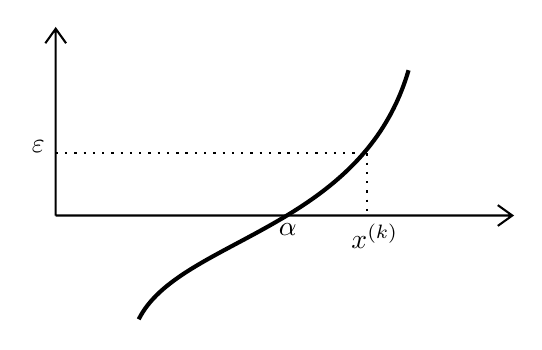
\begin{tikzpicture}[x=0.75pt,y=0.75pt,yscale=-1,xscale=1]
	%uncomment if require: \path (0,160); %set diagram left start at 0, and has height of 160

	%Shape: Axis 2D [id:dp0781238009436287]
	\draw  (170,100) -- (390,100)(170,10) -- (170,100) -- cycle (383,95) -- (390,100) -- (383,105) (165,17) -- (170,10) -- (175,17)  ;
	%Curve Lines [id:da9488325471753964]
	\draw [line width=1.5]    (210,150) .. controls (229.33,111.14) and (317.4,107.4) .. (340,30) ;
	%Straight Lines [id:da7511237307631471]
	\draw  [dash pattern={on 0.84pt off 2.51pt}]  (320,70) -- (320,100) ;
	%Straight Lines [id:da6198333171550376]
	\draw  [dash pattern={on 0.84pt off 2.51pt}]  (170,70) -- (320,70) ;

	% Text Node
	\draw (276,102.4) node [anchor=north west][inner sep=0.75pt]    {$\alpha $};
	% Text Node
	\draw (311,102.4) node [anchor=north west][inner sep=0.75pt]    {$x^{( k)}$};
	% Text Node
	\draw (157,62.4) node [anchor=north west][inner sep=0.75pt]    {$\varepsilon $};


	\end{tikzpicture}
\end{figure}
\FloatBarrier

\item Se $| f'( \alpha )| \ll 1$ allora $\left| e^{( k)}\right| \gg \varepsilon $ e quindi il \textbf{criterio di arresto è inaffidabile}\index{criterio di arresto!inaffidabile}. Si noti in figura come l'errore sia molto piccolo, ma la soluzione sia ancora molto lontana dallo zero.

\begin{figure}[htpb]
	\centering
	\tikzset{every picture/.style={line width=0.75pt}} %set default line width to 0.75pt

	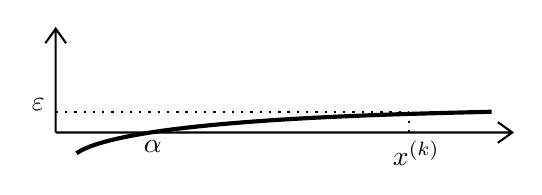
\begin{tikzpicture}[x=0.75pt,y=0.75pt,yscale=-1,xscale=1]
	%uncomment if require: \path (0,99); %set diagram left start at 0, and has height of 99

	%Shape: Axis 2D [id:dp6157046149660421]
	\draw  (180,60) -- (400,60)(180,10) -- (180,60) -- cycle (393,55) -- (400,60) -- (393,65) (175,17) -- (180,10) -- (185,17)  ;
	%Curve Lines [id:da6682504735242709]
	\draw [line width=1.5]    (190,70) .. controls (215,53) and (353.67,51) .. (390,50) ;
	%Straight Lines [id:da3642195964671542]
	\draw  [dash pattern={on 0.84pt off 2.51pt}]  (350,50) -- (350,60) ;
	%Straight Lines [id:da11427175041099624]
	\draw  [dash pattern={on 0.84pt off 2.51pt}]  (180,50) -- (350,50) ;

	% Text Node
	\draw (221,62.4) node [anchor=north west][inner sep=0.75pt]    {$\alpha $};
	% Text Node
	\draw (341,62.4) node [anchor=north west][inner sep=0.75pt]    {$x^{( k)}$};
	% Text Node
	\draw (167,42.4) node [anchor=north west][inner sep=0.75pt]    {$\varepsilon $};


	\end{tikzpicture}
\end{figure}
\FloatBarrier

\item Se $| f'( \alpha )| \gg 1$ allora $\left| e^{( k)}\right| \ll \varepsilon $ e quindi il \textbf{criterio di arresto è troppo stringente}\index{criterio di arresto!troppo stringente}. Si noti in figura il contrario rispetto al punto precedente: l'errore è molto grande anche se la soluzione è molto vicina.

\begin{figure}[htpb]
	\centering
	\tikzset{every picture/.style={line width=0.75pt}} %set default line width to 0.75pt

	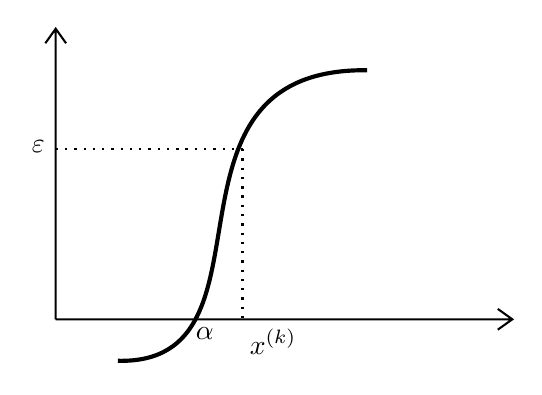
\begin{tikzpicture}[x=0.75pt,y=0.75pt,yscale=-1,xscale=1]
	%uncomment if require: \path (0,201); %set diagram left start at 0, and has height of 201

	%Shape: Axis 2D [id:dp16565494826021832]
	\draw  (180,160) -- (400,160)(180,20) -- (180,160) -- cycle (393,155) -- (400,160) -- (393,165) (175,27) -- (180,20) -- (185,27)  ;
	%Curve Lines [id:da0007870013764332828]
	\draw [line width=1.5]    (210,180) .. controls (292,181.84) and (221,38.84) .. (330,40) ;
	%Straight Lines [id:da25268726559402355]
	\draw  [dash pattern={on 0.84pt off 2.51pt}]  (270,78) -- (270,160) ;
	%Straight Lines [id:da28261351997743933]
	\draw  [dash pattern={on 0.84pt off 2.51pt}]  (180,78) -- (270,78) ;

	% Text Node
	\draw (246,162.4) node [anchor=north west][inner sep=0.75pt]    {$\alpha $};
	% Text Node
	\draw (272,163.4) node [anchor=north west][inner sep=0.75pt]    {$x^{( k)}$};
	% Text Node
	\draw (167,72.4) node [anchor=north west][inner sep=0.75pt]    {$\varepsilon $};


	\end{tikzpicture}
\end{figure}
\FloatBarrier

\end{enumerate}

\subsection{Controllo sull'incremento}
Fissando la tolleranza $\varepsilon  >0$, terminiamo il ciclo quando
\begin{equation*}
\left| x^{( k+1)} -x^{(k)}\right| < \varepsilon.
\end{equation*}
Grazie a uno sviluppo di Taylor possiamo scrivere
\begin{equation*}
e^{( k+1)} =\alpha -x^{( k+1)} =\Phi ( \alpha ) -\Phi \left( x^{( k)}\right) =\Phi '\left( \xi ^{( k)}\right) e^{( k)}
\end{equation*}
allora
\begin{equation*}
x^{( k+1)} -x^{( k)} =e^{( k)} -e^{( k+1)} =\left( 1-\Phi '\left( \xi ^{( k)}\right)\right) e^{( k)}.
\end{equation*}
Dato che $\xi ^{( k)}$ sta convergendo ad $\alpha $ possiamo assumere che $\Phi '\left( \xi ^{( k)}\right) \approx \Phi '( \alpha )$, da cui
\begin{equation}
e^{( k)} =\frac{1}{1-\Phi '( \alpha )}\left( x^{( k+1)} -x^{( k)}\right).
\end{equation}
Quindi:
\begin{itemize}
\item se $\Phi '( \alpha ) \approx 1$ allora il criterio è \textit{inaffidabile};
\item per i metodi del secondo ordine, se $\Phi '( \alpha ) =0$ allora il criterio è \textit{affidabile};
\item continua ad essere soddisfacente se $-1< \Phi '( \alpha ) < 0$.
\end{itemize}

\section{Sistemi di equazioni non lineari}
Vediamo l'estensione vettoriale dello stesso tipo di problema visto nelle pagine precedenti.
Sia assegnata $\mathbf{F} :\mathbb{R}^{n}\rightarrow \mathbb{R}^{n}$: vogliamo trovare $\x^{\star } \in \mathbb{R}^{n}$ tale che $\mathbf{F}\left(\x^{\star }\right) =\mathbf{0}$.

Ricordiamo che la \textbf{matrice jacobiana}\index{matrice!jacobiana} associata a $\mathbf{F}$ e valutata nel punto $\x =( x_{1} ,x_{2} ,\dotsc ,x_{n})^{T}$ è data da:
\begin{equation*}
( J_{\mathbf{F}}(\x))_{ij} =\frac{\partial F_{i}}{\partial x_{j}}(\x) ,\quad i,j=1,\dotsc ,n.
\end{equation*}

Supponiamo anche che $\mathbf{F}$ sia una funzione continua e con derivate parziali positive.
Si ha il seguente algoritmo di punto fisso:

\begin{algo}
	inizializza $\x^{(0)}$\;
	\For{$k=0,1,2,\dotsc$}{
		risolvi $J_{\mathbf{F}}\left(\x^{(k)}\right) \delta \x^{(k)} =-\mathbf{F}\left( x^{(k)}\right)$\;
		aggiorna $\x^{( k+1)} =\x^{(k)} +\delta \x^{(k)}$\;
		\If{criterio di arresto}{
			termina algoritmo\;
		}
	}
	\caption{Algoritmo di Newton per sistemi non lineari.}
\end{algo}
\textit{Osservazione.} Esistono molte varianti di questo algoritmo, ad esempio basate su opportune approssimazioni di $J_{\mathbf{F}}\left(\x^{(k)}\right)$ oppure sull'aggiornamento di $J_{\mathbf{F}}\left(\x^{(k)}\right)$ solo una volta ogni $k^*$ iterazioni, con $k^* > 1$.
\begin{theorem}
[Convergenza di Newton per sistemi non lineari]
Sia $\mathbf{F} :\mathbb{R}^{n}\rightarrow \mathbb{R}^{n}$, $\mathbf{F} \in C^{1}(D)$, dove $D$ è un sottoinsieme aperto convesso di $\mathbb{R}^{n}$ che contiene $\x^{\star }$. Supponiamo inoltre che $J_{\mathbf{F}}\left(\x^{\star }\right)$ sia invertibile, e che esistano delle costanti positive $R,C,L$ tali che $\left\Vert J^{-1}_{\mathbf{F}}\left(\x^{\star }\right)\right\Vert \leqslant C$ e
\begin{equation*}
\Vert J_{\mathbf{F}}(\mathbf{z}) -J_{\mathbf{F}}(\y)\Vert \leqslant L\Vert \mathbf{z} -\y\Vert ,\quad \forall \mathbf{z} ,\y \in B\left(\x^{\star } ,R\right)
\end{equation*}
avendo indicato con lo stesso simbolo $\Vert \cdot \Vert $ una norma vettoriale ed una norma matriciale consistenti\footnote{Una norma matriciale $\Vert \cdot \Vert $ su $\mathbb{R}^{m\times n}$ è consistente con una norma vettoriale $\Vert \cdot \Vert _{a}$ su $\mathbb{R}^{n}$ e $\Vert \cdot \Vert _{b}$ su $\mathbb{R}^{m}$ se $\Vert A\x\Vert _{b} \leqslant \Vert A\Vert \Vert \x\Vert _{a}$ per tutte le matrici $A\in \mathbb{R}^{m\times n}$ e i vettori $\x \in \mathbb{R}^{n}$. Tutte le norme indotte, cioè quelle che consideriamo in questo corso, sono consistenti per definizione.}.
Esiste allora $r >0$ tale che, per ogni $\x^{(0)} \in B\left(\x^{\star } ,r\right)$ il metodo di Newton è univocamente definito, converge a $\x^{\star }$ ed è tale che
\begin{equation*}
\left\Vert \x^{(k+1)} -\x^{\star }\right\Vert \leq CL\left\Vert \x^{(k)} -\x^{\star }\right\Vert ^{2}.
\end{equation*}
\end{theorem}
